\documentclass[a4paper,12pt]{article}
\usepackage[spanish]{babel}
\usepackage[T1]{fontenc}
\usepackage[utf8]{inputenc}
\usepackage{url}
%\usepackage{makeidx}
\usepackage{graphicx}
\usepackage{listings} %Para poner código fuente
\usepackage{ifpdf}
\ifpdf
\usepackage[pdftex,
            pagebackref=true,
            colorlinks=true,
            linkcolor=blue,
            unicode
           ]{hyperref}
\else
\usepackage[ps2pdf,
            pagebackref=true,
            colorlinks=true,
            linkcolor=blue,
            unicode
           ]{hyperref}
\usepackage{pspicture}
\fi
\title{Trabajo final de análisis y diseño de algoritmos I}
\author{Lucas Moauro}
\date{}
\begin{document}
\maketitle
\newpage
\tableofcontents
\section{Introducción}
% * Motivación para el tp.
% * Resúmen de cambios realizados, aclarar que fue reescrito.
% * Sobre Qt y la SDL(aclarar sobre la complejidad temporal de las estructuras).
% * Resúmen de el contenido de cada sección.
En este informe se presentan las modificaciones al programa Clausula que fueron realizadas como trabajo final
para la cátedra \emph{Análisis y diseño de algoritmos I}.

Clausula \cite{Clausula} es un deductor de lógica de primer orden; a partir de una lista de cláusulas es capaz
de determinar su satisfacibilidad. Además, provee otras funciones útiles para el estudio de lógica como la
unificación de literales y la simplificación de un conjunto de cláusulas utilizando diferentes criterios. Estas funcionalidades
son accesibles a través de una interfaz gráfica intuitiva. Este programa es utilizado por los alumnos de la cátedra \emph{Ciencias de la
computación II} dictada en el segundo año de la carrera.

La motivación del trabajo fue agregar optimizaciones y funcionalidades al programa,
a saber:
\begin{itemize}
\renewcommand{\labelitemi}{$\bullet$}
\item La refactorización de las clases básicas(Término, Literal, Cláusula, etc). Se agregaron relaciones
de herencia y se cambiaron de lugar métodos.
\item Se cambió la gramática de las cláusulas permitiendo identificadores de más de un caracter. Se creó una clase
que provee la adición y eliminación de clausulas y el manejo de errores sintácticos y semánticos.
\item Se creó una clase abstracta que sirve de base para las diferentes estrategias de resolución.
\item Los procedimientos de resolución corren en un hilo de ejecución diferente, lo que permite al usuario detener la resolución sin tener que
salir del programa.
\item Se agregó una regla de inferencia(factorización) que es necesaria para la completitud de los métodos de resolución.
\item Se implementó una simplificación conocida como \emph{simplificación por literales eliminables}.
\item Se implementó una simplificación por subsunción de cláusulas.
\item Se implementó una simplificación de la traza de resolución que elimina las inferencias que no fueron
usadas para derivar la cláusula vacía y se agregó un indexamiento de cláusulas. Esto hace que las pruebas sean
más cortas y legibles.
\item Se integró Clausula con un programa para transformar fórmulas a la forma clausular, lo que permite al usuario
determinar la satisfacibilidad de fórmulas arbitrarias.
\item Se separó completamente la interfaz gráfica de los algoritmos y clases fundamentales, de esta forma
pueden usarse sin mayores dependencias en otros proyectos.
\end{itemize}
En este proyecto se usaron extensivamente los contenedores provistos por la STL(listas, mapas, conjuntos, etc). Además
de la especificación formal de cada contenedor, la STL especifica la complejidad temporal asintótica de los métodos de
inserción, eliminación, etc.\cite{sgi}

\section{Estructuras básicas de lógica de primer orden}
%En esta sección tengo que explicar desde el punto de vista de lógica de primer orden
%a los términos(variables y funciones), literales, y cláusulas. Después hay que describir
%las clases utilizadas para representarlos, sin hacer incapié en como están implementados
%los algoritmos, sólo la interfaz externa. También Sustitución y Argumentos.
En esta sección se describen las estructuras básicas de lógica de primer orden que sirven de base para los métodos de resolución.
Primero se introducen a partir de su definición en lógica y luego se plantea la correspondencia a los tipos de datos abstractos
y a su implementación a través de las clases de C++ describiendo los métodos más importantes de cada clase. 
Por último, se dan a conocer las estructuras utilizadas para la representación interna de las clases.

Los principales cambios con respecto a las estructuras de \emph{Clausula} son las relaciones de herencia
en las clases que representan términos, la representación interna y la inclusión de métodos que en Clausula
se encontraban en una clase monolítica llamada \emph{CAlgoritmos}.
\subsection{Términos: Variables y Funciones} %también la clase argumentos
En lógica de primer orden, el conjunto de términos es definido inductivamente \cite{ApuntesLogica}:
\begin{enumerate}
\item Una \emph{variable} es un término.
\item Si $t_1,t_2,...,t_n$ son términos y $f$ es un símbolo de \emph{función}, entonces $f(t_1,t_2,...,t_n)$
  es un término.\footnote{Las constantes son funciones de aridad 0.}
\end{enumerate}
Las variables se caracterizan por tener un identificador y las funciones un identificador y argumentos. La existencia de
dos tipos de términos, sugiere la utilización de un  TDA \emph{Termino} del cual se derivan los TDAs \emph{Variable} y 
\emph{Funcion}.
\begin{center}
\leavevmode
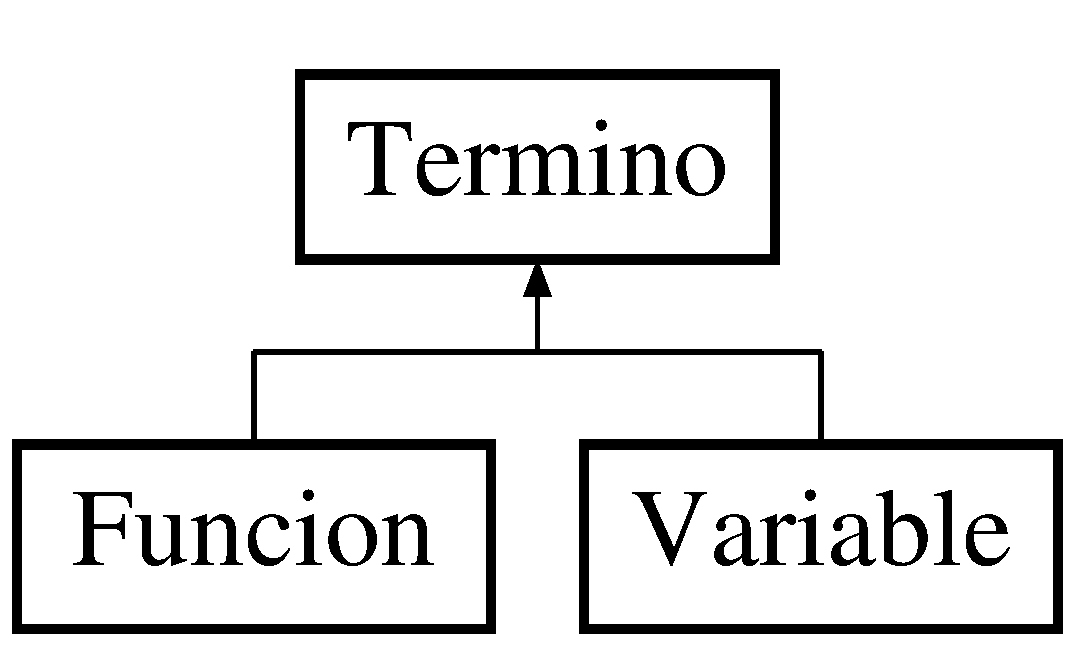
\includegraphics[height=2cm]{imagenes/classTermino}
\end{center}
En la clase abstracta Termino se declaran métodos a ser implementados en sus clases derivadas
\footnote{La documentación detallada de cada método se encuentra en el manual de referencia de clases.}.
\begin{itemize}
\renewcommand{\labelitemi}{$\bullet$}
\item const std::string \& getId () const
\item t getTipo () const
\item virtual const std::string getString () const =0
\item virtual bool operator== (const Termino \&otro) const =0
\item virtual bool contieneVariable (const std::string \&id) const =0
\item virtual Termino $\ast$ aplicarSustitucion (const Sustitucion \&s) const =0
\item virtual bool unificar (Sustitucion \&s, const Termino \&otro) const =0
\item virtual bool unificarSubsuncion (Sustitucion \&s, const Termino \&otro) const =0
\item virtual void renombrarVariables (std::map< std::string, std::string > \&renombre, int \&comienzo)=0
\end{itemize}
La clase Funcion, además de implementar los métodos virtuales de la clase Termino,
provee métodos específicos a las funciones de lógica de primer orden, como el acceso a la aridad
de la función y la adición de argumentos.

Existe otra estructura lógica que posee términos como argumentos, el Literal. Por este motivo, es conveniente
encapsular el concepto de argumentos en una clase que provea funcionalidad para ambas clases. La clase \emph{Argumentos}
cumple este objetivo.
\begin{itemize}
\renewcommand{\labelitemi}{$\bullet$}
\item Argumentos (const Argumentos \&Args)
\item int aridad () const
\item const std::string getString () const
\item const\_iterator begin () const
\item const\_iterator end () const
\item bool operator== (const Argumentos \&otro) const
\item bool contieneVariable (const std::string \&id) const
\item bool unificar (Sustitucion \&s, const Argumentos \&otro) const
\item bool unificarSubsuncion (Sustitucion \&s, const Argumentos \&otro) const
\item void agregarArgumento (const Termino \&t)
\item void aplicarSustitucion (const Sustitucion \&s)
\item void renombrarVariables (std::map< std::string, std::string > \&renombre, int \&comienzo)
\end{itemize}
Para la representación interna de los argumentos en la clase Argumentos se optó por
usar una lista de punteros a objetos de la clase Termino. De esta forma, la inserción de términos
tiene complejidad constante y la utilización de punteros permite que los argumentos sean objetos polimórficos.

Para representar los identificadores de las variables y funciones se usa la clase \emph{string} de la STL.
\subsection{Sustitución}
Una sustitución es una asignación de variables a términos. Estas son utilizadas en la implementación de los
algoritmos de unificación y en el renombre de variables para estandarizar estructuras lógicas.
El TDA debe proveer funciones para la consulta, asignación y composición de sustituciones.
La clase \emph{Sustitucion} implementa el TDA.
\begin{itemize}
\renewcommand{\labelitemi}{$\bullet$}
\item const Termino $\ast$ getSustitucion (const std::string \&id) const
\item void agregarSustitucion (const std::string \&id, const Termino \&t)
\item void componer (const Sustitucion \&s)
\end{itemize}
La estructura interna de la clase esta compuesta por un mapa de la STL en el cual los
índices son identificadores de variables y los valores son punteros a términos. El mapa
provee acceso aleatorio a las sustituciones garantizando una complejidad temporal de 
$O(\log n)$, siendo $n$ la cantidad de sustituciones en el mapa.
\subsection{Literal}
En lógica de primer orden un literal es una fórmula atómica o la negación de una.
Esta caracterizado por tener un signo, identificador y argumentos. Los argumentos
de un literal son términos.
La clase \emph{Literal} provee métodos para el acceso y modificación de un literal. También
implementa métodos que son usados en el cálculo de resolventes, por ejemplo un método que determina
si dos literales son complementarios.
\begin{itemize}
\renewcommand{\labelitemi}{$\bullet$}
\item Literal (const std::string \&id, bool signo)
\item Literal (const std::string \&id, const Argumentos \&args, bool signo)
\item bool getSigno () const
\item const std::string \& getId () const
\item const std::string getString () const
\item int aridad () const
\item bool operator== (const Literal \&otro) const
\item bool operator!= (const Literal \&otro) const
\item const\_iterator begin () const
\item const\_iterator end () const
\item bool unificar (const Literal \&otro, Sustitucion \&s) const
\item bool unificable (const Literal \&otro) const
\item bool unificarComplementario (const Literal \&otro, Sustitucion \&s) const
\item bool unificarSubsuncion (const Literal \&otro, Sustitucion \&s) const
\item void aplicarSustitucion (const Sustitucion \&s)
\item void agregarArgumento (const Termino \&t)
\item void setSigno (bool s)
\item void renombrarVariables (std::map< std::string, std::string > \&renombre, int \&comienzo)
\item void renombrarVariables (int \&comienzo)
\end{itemize}
Como se ha mencionado anteriormente, la estructura interna de los argumentos de la clase
\emph{Literal} está representada por un objeto de la clase \emph{Argumentos}.
\subsection{Cláusula}
Una cláusula es una disyunción de literales. Es la estructura lógica sobre la cual se basan
las estrategias de resolución. La clase \emph{Clausula} implementa esta estructura. Provee operaciones
para la consulta e inserción de literales y para aplicar las dos reglas de inferencia fundamentales en
el cálculo de resolución: el cálculo de resolventes entre dos cláusulas y la factorización de una cláusula.
Un detalle importante es que la clase permite asignar un entero como identificador a una cláusula creada. Los
identificadores son usados para indexar las cláusulas y aplicar simplificaciones a la traza de resolución.
\begin{itemize}
\renewcommand{\labelitemi}{$\bullet$}
\item Clausula (int id\_resolucion=0)
\item int cantLiterales () const
\item bool esUnitaria () const
\item bool esDeHorn (t\_horn \&t) const
\item bool esDeHorn () const
\item bool esVacia () const
\item bool esTautologica () const
\item const std::string getString () const
\item int getIdResolucion () const
\item const\_iterator begin () const
\item const\_iterator end () const
\item bool contieneComplementario (const Literal \&lit) const
\item bool contienePredicado (const std::string \&id\_pred) const
\item bool subsume (const Clausula \&otra) const
\item void resolventes (const Clausula \&claus, std::list< Clausula > \&res) const
\item bool resolventeUsandoPred (const Clausula \&claus, const std::string \&id\_pred, Clausula \&res) const
\item void factores (std::list< Clausula > \&fact) const
\item bool equivalente (const Clausula \&C) const
\item Clausula renombrarVariables (int \&comienzo) const
\item std::map< std::string, int > aparicionesPredicados () const
\item void agregarLiteral (const Literal \&lit)
\item void setIdResolucion (int id)
\end{itemize}
Para la representación interna de los literales se utiliza un set de la STL. La disyunción puede interpretarse como
un conjunto de literales teniendo en cuenta la propiedad de idempotencia, esta indica que una cláusula que contiene
$n$ iguales es equivalente a una cláusula obtenida de eliminar $n-1$ de los $n$ literales iguales. Para poder usar
un set es necesario definir un orden parcial para los literales, este orden está definido en la clase \emph{LitComp}.
El hecho de que los literales se encuentren ordenados permite hacer que varios métodos de la clase sean más eficientes,
ya que al conocer esta propiedad no deben iterar sobre todo el conjunto de literales.
\section{Análisis sintáctico de cláusulas} %gramática y parser.
Para interpretar la entrada de cláusulas es necesario definir una sintaxis concreta para las estructuras
lógicas y de esta forma poder transformar una cadena ingresada a una clase con sus respectivos atributos.
La refactorización de la gramática se hizo por ciertas limitaciones en la gramática de Clausula. También
se creo una clase, \emph{Parser} que encapsula métodos para analizar un conjunto de cláusulas.
\subsection{Gramática}
La principal limitación en la gramática de Clausula es que los identificadores de variables, funciones y literales
están compuestos por un símbolo alfabético, lo que impide que el usuario pueda asignar nombres más significativos. Además,
en problemas no triviales, con una mayor cantidad de identificadores puede que no pueda representarse el problema
usando esa gramática. En la nueva gramática los identificadores pueden contener más de un caracter.

En Clausula es necesario definir que identificadores son símbolos de constantes porque el conjunto
de símbolos posibles para asignar a las variables es igual al de las constantes. Esto se resuelve haciendo
que el conjunto de identificadores para las constantes sea diferente al de las variables; los
identificadores de variables empiezan con una letra mayúscula y los identificadores de literales, funciones y constantes
empiezan con minúscula.

A continuación se define la nueva gramática en formato \emph{BNF}.
%gramática
\lstinputlisting[basicstyle=\small,caption=Gramática, frame=single]{gramatica.bnf}
En cuanto a la implementación, se cambió el uso de \emph{Bison} por el de la biblioteca \emph{Spirit}\cite{spirit}.
El principal motivo es que provee una mejor integración con el lenguaje C++ y la gramática puede usarse como una biblioteca
sin la necesidad de invocar a un programa externo para el análisis sintáctico\footnote{Esto también es posible con Bison pero es más complejo.}.
\subsection{Parser}
La gramática definida en \emph{Spirit} detecta los posibles errores sintácticos en la definición
de una cláusula pero no los errores semánticos. Existen dos posibles errores semánticos:
\begin{enumerate}
\item Un identificador de función o predicado es usado con diferentes aridades. Por ejemplo, $a(X) \lor a(X,Y)$ no
es una cláusula bien definida.
\item Un identificador es usado para identificar a una función y a un predicado. Por ejemplo $a(a(X))$ no es válida.
\end{enumerate}
Estos errores semánticos pueden ser errores dentro de una misma cláusula o puede que sean producto de una
inconsistencia entre dos o más cláusulas. La clase \emph{Parser} es la encargada de analizar incrementalmente
un conjunto de cláusulas, verificando la validez del conjunto cada vez que se agrega o elimina una cláusula.
Esta clase es usada como modelo de datos en la interfaz gráfica que acepta cadenas ingresadas por el usuario.
\begin{itemize}
\renewcommand{\labelitemi}{$\bullet$}
\item void parseClausula (int id, const std::string \&clausula, bool \&error, std::pair< t\_error, std::string >\&E)
\item void eliminarClausula (int id)
\item Clausula getClausula (int id) const
\item void getClausulas (std::list< Clausula > \&l) const
\item void getClausulas (ConjuntoClausulas<> \&claus) const
\end{itemize}
En la representación interna de las cláusulas se usa un mapa de enteros a cláusulas, los enteros
son identificadores provistos por el cliente de la clase para después poder consultar una cláusula
del conjunto o eliminarla. También se utilizan mapas de tipo y aridad para la verificación semántica
de las cláusulas.
\section{Factorización de cláusulas}
La regla de inferencia de factorización\cite{PracticalLogic} es necesaria para que los métodos de
resolución sean refutacionalmente completos. En Clausula esta regla no esta presente por lo que
para ciertos conjuntos de cláusulas insatisfacibles no consigue derivar la cláusula vacía.

A modo de ejemplo puede considerarse el siguiente conjunto de cláusulas:
\begin{enumerate}
\item $s(X,X)\lor s(b,X)$
\item $\lnot s(Y,Y)\lor \lnot s(b,Y)$
\end{enumerate}
Este conjunto puede probarse insatisfacible usando modelos de Herbrand pero no es posible
derivar la cláusula vacía usando sólo la regla de la resolvente como se muestra a continuación.
\begin{enumerate}
\item $s(X,X)\lor s(b,X)$
\item $\lnot s(Y,Y)\lor \lnot s(b,Y)$
\item $Res(1,2) \equiv s(b,X) \lor \lnot s(b,X) \equiv T$ usando la sustitución \{Y/X\} y los
literales $s(X,X)$ y $\lnot s(Y,Y)$ como complementarios.
\item $Res(1,2) \equiv s(X,X) \lor \lnot s(Y,Y) \equiv T$ usando la sustitución \{Y/X\} y los
literales $s(b,X)$ y $\lnot s(b,Y)$ como complementarios.
\end{enumerate}
La regla de factorización consiste en unificar dos literales en una cláusula y crear una nueva
cláusula aplicando la sustitución que unifica a esos dos literales. Utilizando esta regla puede
derivarse la cláusula vacía en el ejemplo anterior.
\begin{enumerate}
\item $s(X,X)\lor s(b,X)$
\item $\lnot s(Y,Y)\lor \lnot s(b,Y)$
\item $Factor(1) \equiv s(b,b)$ \{X/b\}
\item $Factor(2) \equiv \lnot s(b,b)$ \{Y/b\}
\item $Res(3,4) \equiv \bot$
\end{enumerate}
El algoritmo de factorización está implementado en la clase Clausula, en el método
Clausula::factores, este inserta los factores de la cláusula a una lista pasada
por referencia.
\lstinputlisting[caption=Factores, frame=single, numbers=left,language=C++,basicstyle=\tiny]{factores.cpp}
La complejidad del algoritmo es determinada por los ciclos anidados en las lineas 3, 6 y 10. Estos iteran
sobre los literales de la cláusula, por lo que la complejidad es de $O(n^3)$, siendo $n$ la cantidad de
literales de la cláusula.%FIX
\section{Estructuras de resolución}
En esta sección se presentan las clases usadas para la determinación de la satisfacibilidad
de cláusulas.
\subsection{ConjuntoClausulas}
La clase \emph{ConjuntoClausulas} representa un conjunto de cláusulas. Provee métodos
para la simplificación y la determinación de propiedades del conjunto.
\begin{itemize}
\renewcommand{\labelitemi}{$\bullet$}
\item template<typename Iterator > ConjuntoClausulas (Iterator begin, Iterator end, bool numerar=false)
\item size\_type cantidadClausulas () const
\item bool esVacio () const
\item bool esDeHorn () const
\item bool esLogicaPrograma () const
\item void agregarClausula (const Clausula \&C)
\item bool simplificarPorTautologicas ()
\item bool simplificarPorEquivalentes ()
\item bool simplificarLiteralesPuros ()
\item bool contieneClausula (const Clausula \&c) const
\item void getClausulas (std::list< Clausula > \&l) const
\item std::set< std::string > predicadosEliminables () const
\item const\_iterator begin () const
\item const\_iterator end () const
\item iterator begin ()
\item iterator end ()
\item void eliminar (iterator c)
\end{itemize}
Para representar el conjunto de cláusulas, se usa un set de la STL.

En las estrategias de resolución es útil poder definir mas de un orden parcial para el ordenamiento de
las cláusulas. Por este motivo la clase \emph{ConjuntoClausulas} fue implementada con un template que
permite parametrizar el orden parcial a utilizar. El orden que se utiliza por defecto ordena las cláusulas
en por cantidad de literales en forma creciente.
\subsection{Inferencia}
La traza de resolución es la secuencia de reglas de inferencia aplicadas para derivar la cláusula
vacía. Esta información debe ser provista al usuario con fines didácticos. 

La clase abstracta \emph{Inferencia} representa la aplicación de una regla de inferencia. Entre sus atributos se encuentran
las cláusulas que se usaron en la aplicación de la regla(\emph{padres}) y la cláusula obtenido. A partir de
la clase inferencia se derivan tres clases: \emph{InferenciaHipotesis}\footnote{Las hipótesis no son teóricamente
inferencias, se cuentan como inferencias en este caso para lograr una mayor generalización.}, \emph{InferenciaResolucion} e
\emph{InferenciaFactorizacion}.
\begin{center}
\leavevmode
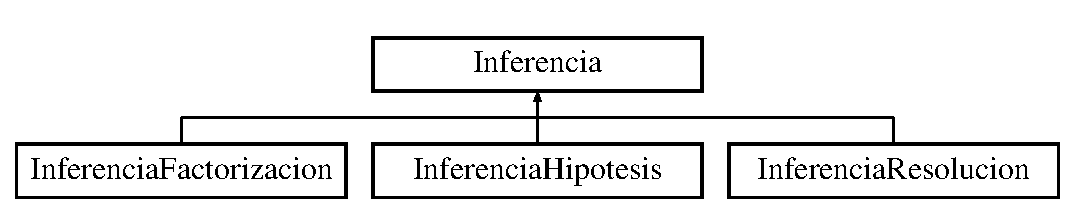
\includegraphics[height=2cm]{imagenes/classInferencia}
\end{center}
\begin{itemize}
\renewcommand{\labelitemi}{$\bullet$}
\item Inferencia (const Clausula \&cl)
\item virtual t\_inf getTipo () const =0
\item const Clausula \& getClausula () const
\item virtual void getPadres (std::list< int > \&) const =0
\item virtual void setPadres (const std::list< int > \&)=0
\end{itemize}
Un detalle importante en la representación interna es que se usan los identificadores(enteros) de los padres
y no las cláusulas. De esta forma puede armarse el árbol de derivación de una inferencia, que es
necesario para la simplificación de la traza.
\subsection{Resolución}
En la verificación de satisfacibilidad de fórmulas existen diferentes estrategias de resolución que pueden
aplicarse según las propiedades del conjunto de cláusulas a analizar. Las dos implementadas en este
trabajo son las estrategias de resolución general y resolución unitaria. La existencia de otras estrategias
(por ejemplo, resolución linear) además de estas dos, hace conveniente la generalización de una estrategia de
resolución, para dar una interfaz común y definir métodos comunes a todas.

La clase abstracta \emph{Resolucion} representa una estrategia de resolución; está provista de métodos a 
implementar por las clases derivadas para determinar la satisfacibilidad de un conjunto de cláusulas. 
Además implementa métodos protegidos de simplificación que son utilizados por las clases derivadas \emph{ResolucionGeneral}
y \emph{ResolucionUnitaria}.
\begin{center}
\leavevmode
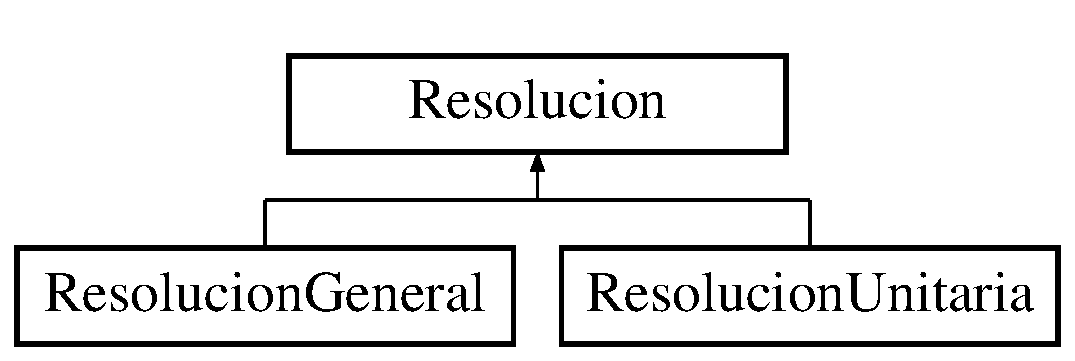
\includegraphics[height=2cm]{imagenes/classResolucion}
\end{center}
\begin{itemize}
\renewcommand{\labelitemi}{$\bullet$}
\item Resolucion (const ConjClaus \&claus)
\item virtual bool esSatisfacible (t\_prueba \&Prueba, const bool \&seguir\_busqueda)=0
\item virtual bool esSatisfacible (t\_prueba \&Prueba)=0
\end{itemize}
El tipo \emph{t\_prueba}, definido dentro de la clase Resolucion, se usa para contener la traza de
resolución. Este es un vector de punteros a objetos de la clase Inferencia, se usa un vector porque
es necesario acceder aleatoriamente a las inferencias para construir el árbol de resolución.
\section{Métodos de resolución}
En esta sección se describen las estrategias de resolución en términos generales. La implementación
de las estrategias están basadas en el ciclo \emph{DISCOUNT}\cite{Schultz} que es utilizado
en otros deductores.

La determinación de la satisfacibilidad de un conjunto de cláusulas es indecidible en general(es decidible 
para cláusulas insatisfacibles), por lo que para ciertas entradas los
procedimientos de resolución no retornaran.
\subsection{Resolución general}
En esta estrategia se intenta derivar la cláusula vacía, mediante un proceso de búsqueda
que genera nuevas cláusulas a partir de las hipótesis. El \emph{estado} de la prueba esta
determinado por el conjunto de cláusulas formado por las hipótesis y las cláusulas obtenidas de la aplicación de 
reglas de inferencia. El proceso es exitoso si se logra derivar la cláusula
vacía(verificando la insatisfacibilidad del conjunto), o si a través de simplificaciones se verifica la satisfacibilidad del conjunto.

La principal dificultad en la implementación de la búsqueda reside en que el estado de prueba crece
muy rápidamente a medida que aumenta la cantidad de inferencias realizadas. Por este motivo es importante
implementar simplificaciones que sean capaces de reducir la redundancia de las inferencias generadas.

Para que el método implementado sea completo, eventualmente deben considerarse todas las combinaciones
de cláusulas no redundantes para la aplicación de reglas de inferencia. Para evitar repeticiones en
la combinación de cláusulas el estado de la prueba se divide en dos subconjuntos: el conjunto $P$ de
cláusulas \emph{procesadas} y el conjunto $C$ de cláusulas combinables. Se mantiene la invariante de que
todas las inferencias necesarias entre cláusulas de $P$ ya han sido generadas.

En términos generales, el algoritmo consiste en tomar una cláusula de $C$, realizar todas las inferencias
entre esta cláusula y las de $P$(añadiendo las cláusulas deducidas a $C$) e insertarla en $P$. Este proceso
es repetido hasta que se deriva la cláusula vacía(determinando la insatisfacibilidad del conjunto) o hasta
que $C$ no contiene más cláusulas(determinando la satisfacibilidad del conjunto).

A continuación se muestra el pseudocódigo del método de resolución general.
\begin{lstlisting}[caption=esSatisfacible, frame=single, numbers=left, basicstyle=\tiny]
U = { }
C = ConjHipotesis // el conjunto inicial de combinables son las hipotesis
C = resolverPredicadosEliminables(C) //simplificacion por literales eliminables
if (C.contieneVacia())
    return false
satisfacible = true
while (satisfacible && C != { }) {
    combinable = C.begin()
    fact = factores(combinable)
    C = agregarFactores(fact, C)
    procesada = P.begin()
    while (satisfacible && procesada != P.end()) {
        res = resolventes(combinable, procesada)
        C = C + {res}
        if (res.contieneVacia())
            satisfacible = false
        ++procesada
    }
    C = C - {combinable}
    P = P + {combinable}
    ++combinable
}

return satisfacible
\end{lstlisting}
\subsection{Resolución unitaria}
La estrategia de resolución unitaria, es más restrictiva que la de resolución general. Es completa
para conjuntos de cláusulas de \emph{Horn}. Una cláusula es de Horn si tiene como máximo un literal
positivo.

La resolución unitaria agrega la restricción de que para cada regla de la resolvente aplicada debe
intervenir una cláusula unitaria(cláusula que tiene un sólo literal).

Para la implementación de la resolución unitaria es necesario la verificación de la
existencia de cláusulas unitarias en $P \cup C$. Esta tarea resulta eficiente considerando
que los conjuntos que forman el estado de la prueba se encuentran ordenados crecientemente por
la cantidad de literales.
\section{Simplificaciones}
Clausula aplica simplificaciones al conjunto inicial de cláusulas que reducen la cantidad
de inferencias a considerar. El problema surge cuando un conjunto inicial de cláusulas satisfacibles
pasa todas las simplificaciones, sin reducirse hasta el conjunto vacío(por definición, satisfacible). En
este caso las simplificaciones implementadas en los métodos de resolución no son suficientemente efectivas
para evitar que el espacio de búsqueda crezca indefinidamente.

Se implementaron tres algoritmos de simplificación que extienden la cantidad de conjuntos iniciales que
pueden resolverse y reducen la cantidad de reglas de inferencia a aplicar para determinar la satisfacibilidad
de un conjunto.
\subsection{Simplificación por predicados eliminables}
La simplificación por predicados eliminables\cite{Gelperin} consiste en eliminar por completo predicados del conjunto
inicial resolviendo entre cláusulas que contienen dichos predicados. Un predicado es \emph{eliminable} en un
conjunto de cláusulas si no aparece en más de una ocasión en una misma cláusula. Por ejemplo, en el conjunto
de cláusulas $\{p(X,X) \lor q(Y), q(X) \lor \lnot p(X,X) \lor \lnot p(X,Y)\}$, $q$ es eliminable y $p$ no lo es.

Sea $I$ el conjunto inicial de cláusulas y $p$ un predicado eliminable en $I$. El conjunto simplificado $S$
se define por:

 $S = \{c \in I : (p \notin c)\} \cup \{resolvente(c_1,c_2,p) : c_1,c_2  \in I, p\in c_1, p\in c_2\}$

es decir, está formado por todas las cláusulas de $I$ que no contienen a $p$ y todas las resolventes
entre dos cláusulas que contienen $p$ usando ese mismo predicado para la resolución. Como $p$ no aparece en más de una ocasión en una cláusula,
el conjunto $S$ no contiene ninguna cláusula que lo contenga. El teorema de la distribución\cite{Gelperin} afirma que $I$ es 
satisfacible si y sólo si $S$ lo es. Esta simplificación se aplica hasta que no queden mas predicados eliminables.

A modo de ejemplo, puede considerarse el conjunto inicial de cláusulas 

\begin{center} 
$I = \{a(X),\lnot a(X) \lor c(X) \lor d(Y), \lnot c(Y) \lor \lnot d(Y)\}$\footnote{Clausula no lo resuelve.}.
\end{center}

Usando el predicado eliminable ``a'' se obtiene

\begin{center}
$S_1 = \{c(X) \lor d(Y), \lnot c(Y) \lor \lnot d(Y)\}$
\end{center}
luego, usando ``c''
\begin{center}
$S_2 = \{d(X) \lor \lnot d(Y)\}$
\end{center}
El conjunto simplificado puede determinarse satisfacible, ya que no es posible aplicar mas
reglas de inferencia.

La implementación de esta simplificación está implementada en la clase \emph{Resolucion} en los métodos
\emph{eliminarPredicado} y \emph{resolverPredicadosEliminables}.

A continuación se presenta el pseudocódigo del método \emph{eliminarPredicado}:
\begin{lstlisting}[caption=eliminarPredicado, frame=single, numbers=left, basicstyle=\tiny]
eliminarPredicado(I, p) {
    S = { }
    for (lit in I) {
        if (lit.contienePredicado(p)) {
            lit2 = lit
            lit2++
            while (lit2 != I.end()) {
                res = resolvente(lit, lit2, p)
                if (res)
                    S = S + {res}
                lit2++
            }
        } else
            S = S + {lit}
    }
    return S
}
\end{lstlisting}
En el peor de los casos se debe resolver entre todo par de cláusulas, por lo que la complejidad
temporal del algoritmo es de $O(k^2)$ siendo $k$ la cantidad de cláusulas del conjunto $I$.

En el método \emph{resolverPredicadosEliminables} se eliminan predicados eliminables hasta que no 
quede ninguno:
\begin{lstlisting}[caption=resolverPredicadosEliminables, frame=single, numbers=left, basicstyle=\tiny]
resolverPredicadosEliminables(I) {
    S = I
    eliminables = I.predicadosEliminables() //retorna los predicados eliminables O(n),
                                            //n clausulas
    while (eliminables != { }) {
        p = eliminables.begin()
        S = eliminarPredicado(S, p)
        eliminables = I.predicadosEliminables()
    }
    return S
}
\end{lstlisting}
El peor de los casos ocurre cuando se todos los predicados terminan siendo eliminables. Sea $c$ la cantidad
de predicados en el conjunto $I$ y $n$ la cantidad de cláusulas, la complejidad temporal del algoritmo es de
$O(c*n^2)$.
\subsection{Simplificación por subsunción}
En lógica proposicional, una cláusula $C$ subsume a otra cláusula $D$ si $C$ implica lógicamente
$D$. Esto ocurre cuando(sintácticamente) $C\subseteq D$.

En lógica de primer orden, la validez de la implicación entre cláusulas es indecidible\cite{PracticalLogic},
por lo que se adopta una definición mas simple: una cláusula de lógica de primer orden $C$ subsume a otra
cláusula $D$, si existe una sustitución $s$, tal que $C.s\subseteq D$. Si $C$ subsume a $D$, 
entonces $C$ implica lógicamente $D$ pero la reciproca no es válida.

Por ejemplo, sea $C=\{a(Y)\}$\footnote{Se usa la notación de conjuntos para las cláusulas.} y $D=\{a(X),c(Y)\}$, 
tomando $s=\{Y/X\}$, $C$ subsume a $D$ porque $C.s=\{a(X)\}\subseteq D$.

En la simplificación por subsunción si una cláusula $C$ subsume a otra cláusula $D$ se considera
que $C$ es más general que $D$. De este modo, cuando se deriva una cláusula nueva,
si alguna cláusula presente en el estado de búsqueda la subsume, la cláusula derivada
puede descartarse.

Esta simplificación hace más efectiva la búsqueda, eliminando cláusulas que son redundantes y
permite resolver conjuntos satisfacibles que no contienen literales eliminables. Por ejemplo el
conjunto
\begin{center}
$\{a(X) \lor  a(Y),\lnot a(X) \lor  \lnot a(Z) \lor  c(X) \lor  c(Z) \lor  d(U) \lor  d(Y),
\lnot c(X) \lor  \lnot c(Y) \lor  \lnot d(X) \lor  \lnot d(Y)\}$
\end{center}
es determinado satisfacible gracias a la simplificación por subsunción.

Para implementar la prueba de subsunción es necesario un procedimiento simplificado
de unificación de términos. En donde sólo se sustituyen las variables de uno de los términos,
y las variables del del par se consideran distintas incluso si sus identificadores son iguales.
Esto último implica que no es necesario renombrar las variables antes de la unificación y que las sustituciones
aparentemente triviales $x \rightarrow x$ deben ser incluidas.

El problema de la subsunción es NP-completo. En la implementación se usa \emph{backtracking}
intentando unificar dos literales en cada estado, hasta que no queden literales por unificar.
Si bien no es posible realizar podas durante la ejecución del backtracking, se implementó
una verificación antes de su ejecución.
La verificación se basa en la propiedad de que si $C$ subsume a $D$ entonces todos los predicados(identificadores)
de $C$ se encuentran en $D$. La complejidad temporal de esta verificación es polinomial.

A continuación se presenta el código de los dos métodos en la clase \emph{Clausula} que implementan
el algoritmo de subsunción.
\lstinputlisting[caption=subsume, frame=single, numbers=left,language=C++,basicstyle=\tiny]{subsume.cpp}

Es posible determinar la complejidad temporal del algoritmo, calculando el tamaño del espacio de búsqueda.
Sea $C_1 = \{l_{11}...l_{1n}\}$ y $C_2 = \{l_{21}...l_{2n}\}$ las cláusulas de entrada con $n$ y $m$ literales respectivamente. 
El algoritmo intenta unificar literales de $C_1$ con literales de $C_2$, en consecuencia, una solución es una función
de los literales de $C_1$ a los de $C_2$. La cantidad de soluciones que existen en $C_1 \times C_2$ es $m^n$(puede que las funciones no sean inyectivas).
Entonces, la complejidad temporal del algoritmo de subsunción es de $O(m^n)$.
\subsection{Simplificación de la traza}
\bibliographystyle{plain}
\bibliography{doc}
\end{document}
